\section{Testing}
Testing was a key process in the development of the final product just as it was in previous submission. Testing was particular important to determine whether the final system meets the requirements initially set. As well as testing each module individually, further tests were done upon completing the system through integration with the front-end and machine learning systems.

\subsection{Using Mocha and Postman}
The JavaScript framework Mocha was still used in the testing process for modules. The test-suite for our project had some major work done since the last submission, allowing tests to run on the Gitlab server as well as addressing bugs in the test-suite and implementation. Whilst also using Mocha for Unit tests, it was used to test the individual routes and their response whilst comparing them to a template. The same method was applied to test requests. This automation increased the efficiency of production, however, the small amount of routes to test allowed us to be more thorough by manually sending requests to the server using Postman. Postman is a API development tool which allows requests to be sent through an easily manageable user interface. By doing this, expected values were easy to match with actual values, and further bugs could be caught even when the templates had matched previously.

\subsection{Integration Testing}
Once the system had been fully implemented and tested, it was necessary to integrate with the rest of the system such as user interface and the machine learning servers. This allowed us to determine whether specific protocols were implemented correctly and to ensure that all the requirements set by the client were met. To begin the integration process, the server was hosted through the St Andrews web service which allows content to be hosted through the web. This was done by configuring an \textit{nginx} proxy that would allow binding of the loopback address and port number. Using \texttt{tmux}, the session was hosted persistently as it allows terminal sessions to be detached and run in the background. The server runs on the domain \textit{har4.host.cs.st-andrews.ac.uk}. From here, it was possible for other teams to send requests to the running server.
\subsubsection{CORS}
Integration testing also gave the opportunity to find additional errors specifically caused by the linking of servers. An example of this is the realisation of the lack of Cross-Origin support. The running server could not function properly as content requests were being sent to different origins and for security reasons this is not permitted. To fix this additional features were required to be implemented to support CORS. Specifically certain headers were added to permit different origin access.
\subsection{Stress Testing}
Near towards the end, a small duration of time was spent testing the robustness of the final system. This was done using different stress testing tools. First a virtual environment was created to host the server. This was to prevent any side effects that may occur to other processes and users. Once the environment was created, the server was started. The tools that were used included the \textit{Metasploit Framework}, which included multiple \textit{DoS} attack methods. This was designed to test extreme but common cases. In particular, the \textit{TCP synFlood} method was used as it is a very common technique occurring over the internet. It attacks the server during its three-way handshake, the process in which \textit{syn}s are sent and \textit{acknowledgements} are received. \textit{synFlood} essentially sends a succession of \textit{syn} requests, attempting to consume server resources. After conducting the attack, no noticeable effect on performance could be seen, demonstrating that the server could withstand simple TCP based \textit{DoS} attacks.

More tests were conducted in a similar manner. \texttt{slowhttptest} was another tool used in testing the robustness of the system as shown in \ref{fig:stress}. This allowed attacks such as \textit{slowloris} and \textit{slowmessagebody}. These exploit the HTTP protocol as all requests are required to be completely received before they are processed. If the request has not been completely received then the server uses its resources waiting for the rest of the data. A denial of service occurs if too many of these resources are kept busy. Again, after attacking the system with this method, no visible drop in performance could be noticed. With the \textit{slowhttptest} tool, the results of the test were outputted to a \texttt{.csv} file and visualized in a web document. These results provide evidence to the robustness of the server. This can be seen in the folder \texttt{test/stressTest}.

\begin{figure}[H]
	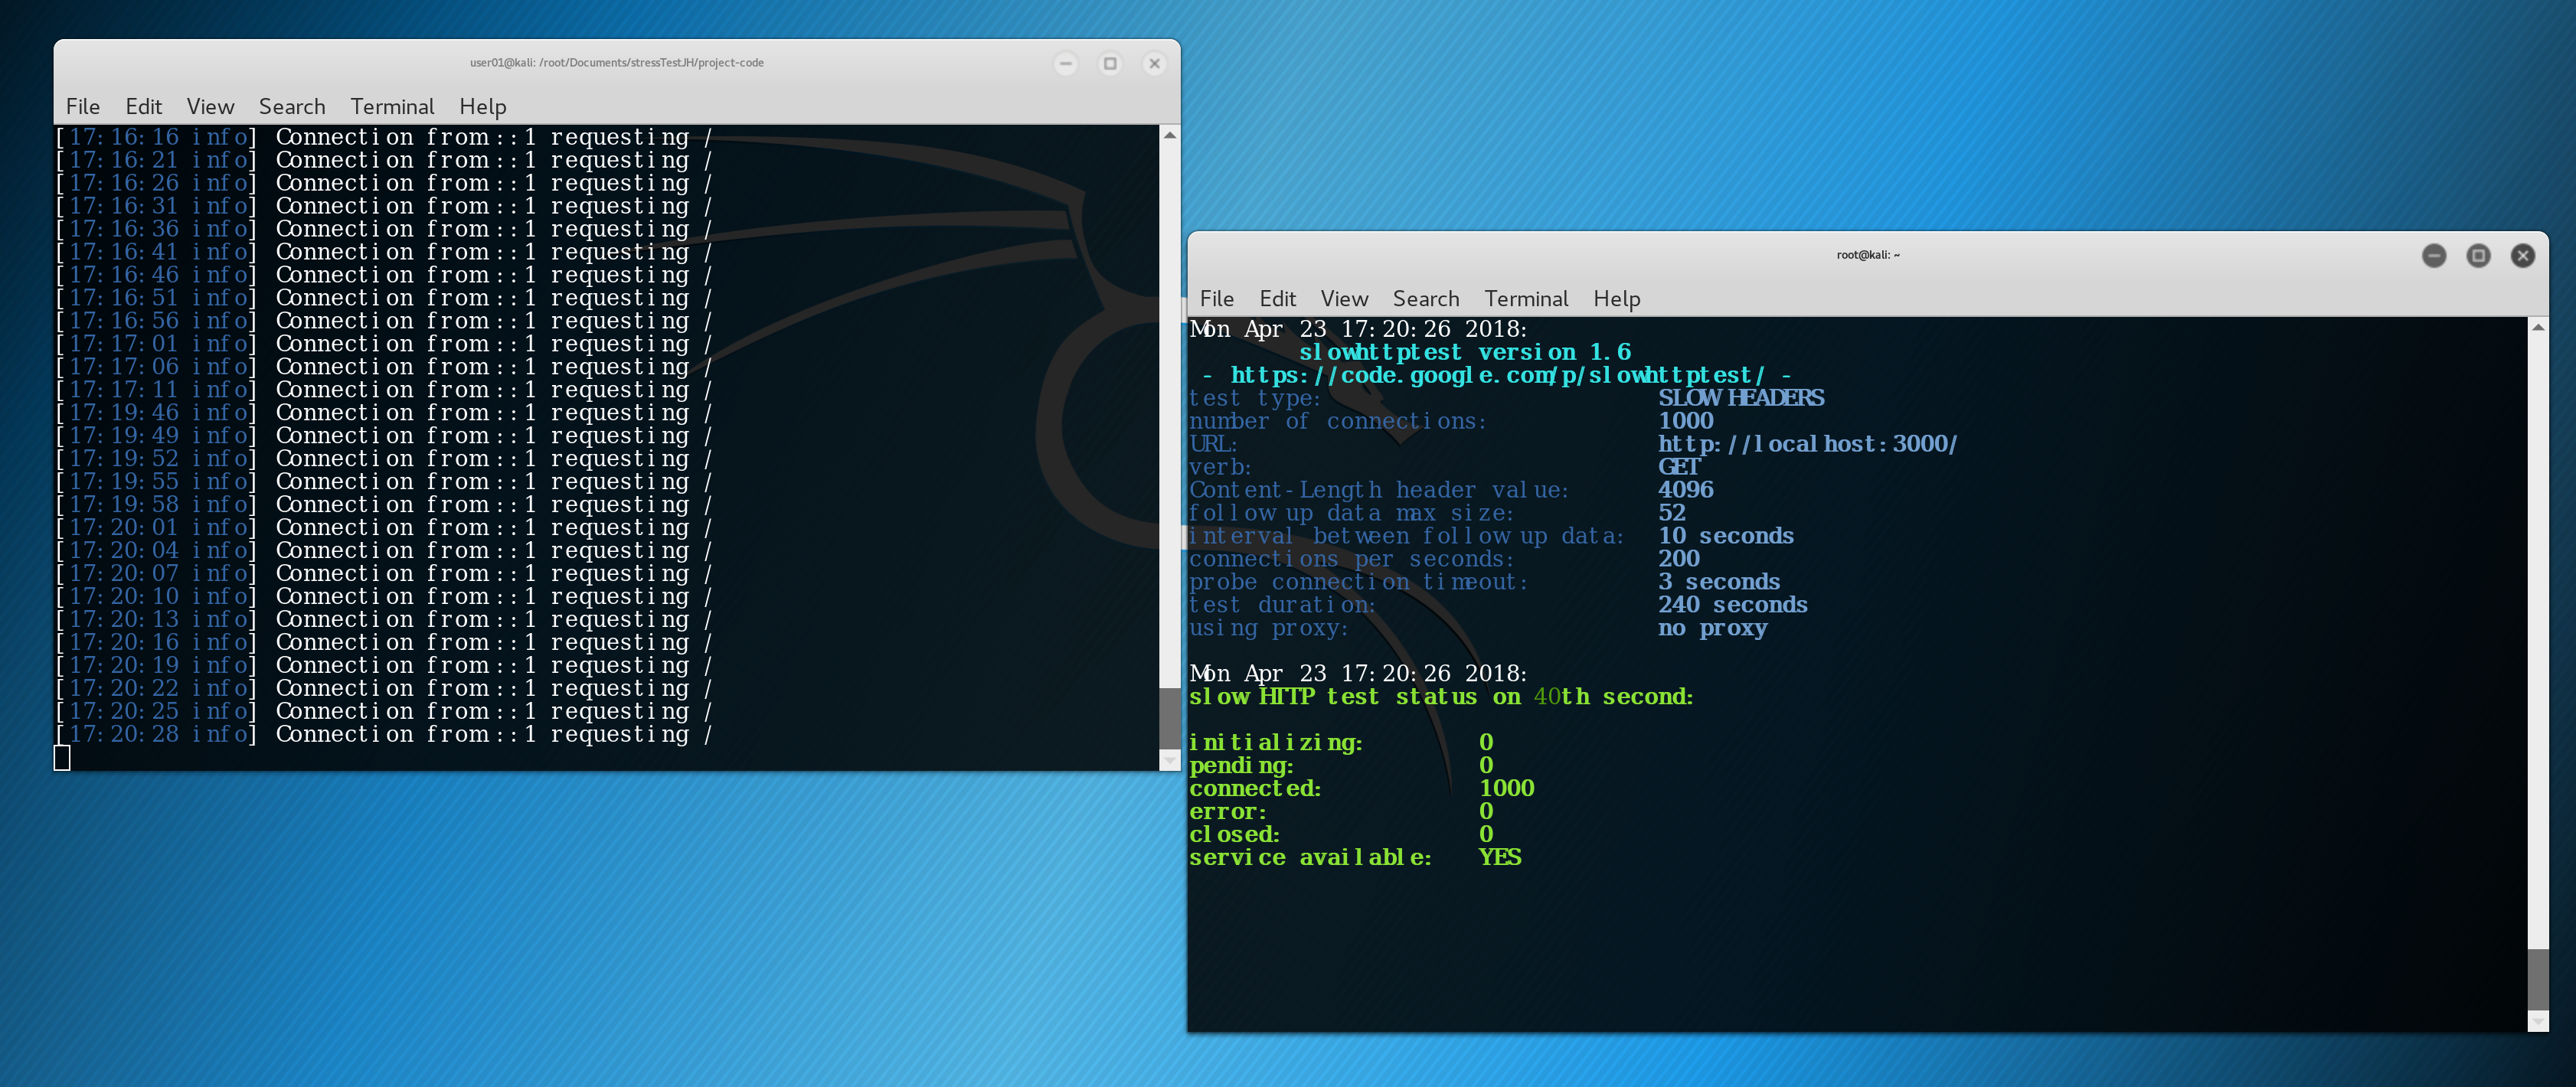
\includegraphics[scale=0.4]{server_tests.png}
	\centering
	\caption{slowhttptest in action}
	\label{fig:stress}
\end{figure}
